\section{Zusammenstellung Signalformen}
\begin{table}[htdp]
\begin{center}
\begin{tabular}{|c|c|c|c|c|}

\hline
\textbf{Signal} & \textbf{$   X_0   $} & \textbf{$X^2$} & \textbf{var(X)} \\
\hline
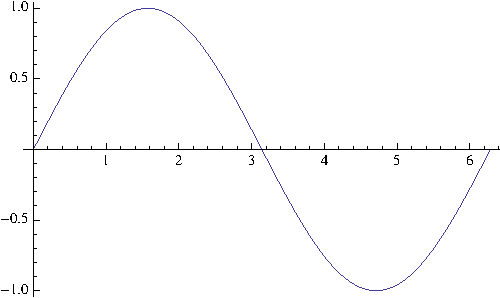
\includegraphics[height=2cm]{./bilder/Sinus.pdf} & $0$ & $\frac{A^2}{2}$ &
$\frac{A^2}{2}$ \\
\hline
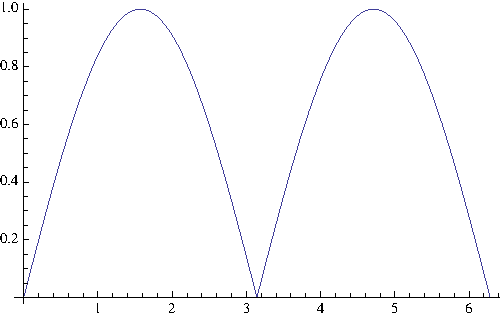
\includegraphics[height=2cm]{./bilder/absSinus.pdf}  & $\frac{2A}{\pi}$ &
$\frac{A^2}{2}$ & $\frac{A^2}{2}-\frac{4A^2}{\pi^2}$\\
\hline
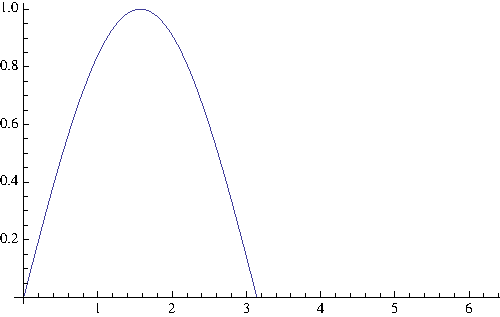
\includegraphics[height=2cm]{./bilder/halbSinus.pdf} & $\frac{A}{\pi}$ &
$\frac{A^2}{4}$ & $\frac{A^2}{4}-\frac{A^2}{\pi^2}$\\
\hline
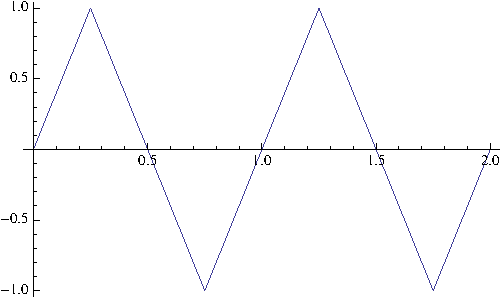
\includegraphics[height=2cm]{./bilder/triangular.pdf} & $0$ & $\frac{A^2}{3}$ &
$\frac{A^2}{3}$ \\
\hline
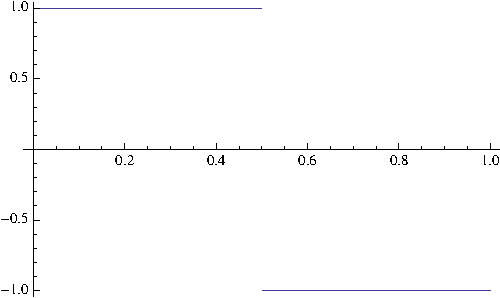
\includegraphics[height=2cm]{./bilder/square.pdf} & $0$ & $A^2$ & $A^2$ \\
\hline
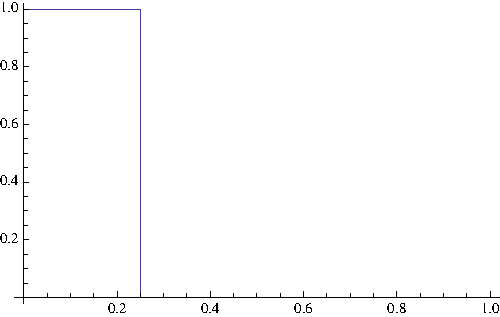
\includegraphics[height=2cm]{./bilder/pwm.pdf}  & $A\frac{t}{T}$ &
$A^2\frac{t}{T}$ & $\frac{A^2t}{T}-\frac{A^2t^2}{T^2}$ \\
\hline

\end{tabular}
\end{center}
\label{default}
\end{table}